\documentclass[tikz,border=10pt]{standalone}
% Trapezoid ABCD; scale s = 0.019139 cm/px, origin at image centre (233, 91.5)
\begin{document}
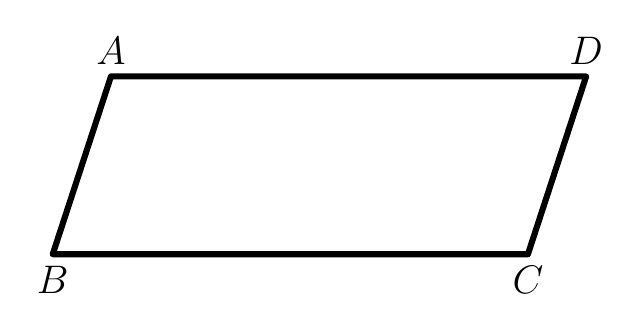
\begin{tikzpicture}[line width=2.2pt, line join=round]
  % Vertices (converted from pixel coordinates, y flipped)
  \coordinate (A) at (-2.663624999995083,1.1387999998973373);
  \coordinate (D) at (3.371425000003349,1.138799999919732);
  \coordinate (B) at (-3.403275000003904,-1.1195999999197568);
  \coordinate (C) at (2.6317749999956384,-1.1195999998973118);

  % Sides AB, BC, CD, DA: solid black, no marks
  \draw[black] (A) -- (B) -- (C) -- (D) -- cycle;

  % Labels just outside each vertex
  \node[above, font=\fontsize{15.5}{18.6}\selectfont] at (A) {$A$};
  \node[above, font=\fontsize{15.5}{18.6}\selectfont] at (D) {$D$};
  \node[below, font=\fontsize{15.5}{18.6}\selectfont] at (B) {$B$};
  \node[below, font=\fontsize{15.5}{18.6}\selectfont] at (C) {$C$};
\end{tikzpicture}
\end{document}